\documentclass{standalone}
\usepackage{tikz}
\begin{document}
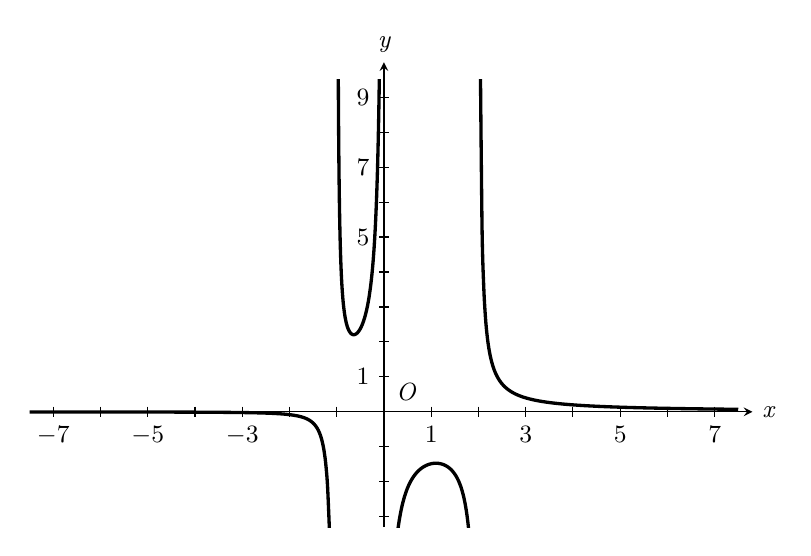
\begin{tikzpicture}[color=black, >=stealth, scale=0.6, y=0.74cm]
  % Axes
  \draw[->] (-7.5,0) -- (7.8,0);
  \draw[->] (0,-3.3) -- (0,10);
  \node[font=\small\itshape, anchor=west] at (7.8,0) {x};
  \node[font=\small\itshape, anchor=south] at (0,10) {y};
  \node[font=\small\itshape, anchor=south west] at (0.05,0.05) {O};
  % x ticks at every integer; labels at -7, -5, -3, 1, 3, 5, 7
  \foreach \x in {-7,...,-1,1,2,...,7}
    \draw (\x,0.15) -- (\x,-0.15);
  \foreach \x in {-7,-5,-3}
    \node[font=\small, anchor=north] at (\x,-0.15) {$\x$};
  \foreach \x in {1,3,5,7}
    \node[font=\small, anchor=north] at (\x,-0.15) {$\x$};
  % y ticks at every integer; labels at 1, 5, 7, 9
  \foreach \y in {-3,...,-1,1,2,...,9}
    \draw (-0.1,\y) -- (0.1,\y);
  \foreach \y in {1,5,7,9}
    \node[font=\small, anchor=east] at (-0.1,\y) {$\y$};
  % Curve: vertical asymptotes at x = -1, 0, 2; horizontal asymptote y = 0
  \begin{scope}
    \clip (-7.5,-3.3) rectangle (7.6,9.5);
    % x < -1: flat along y = 0, then down to -infinity at x = -1
    \draw[line width=1.2pt, smooth, samples=150, domain=-7.5:-1.15]
      plot (\x, {-0.08/((\x+1)^2)});
    % -1 < x < 0: U shape, minimum near (-0.64, 2.2)
    \draw[line width=1.2pt, smooth, samples=150, domain=-0.97:-0.09]
      plot (\x, {0.286/(\x+1) + 0.904/(-\x)});
    % 0 < x < 2: inverted U, maximum near (1.1, -1.5)
    \draw[line width=1.2pt, smooth, samples=150, domain=0.26:1.8]
      plot (\x, {-(0.889/\x + 0.595/(2-\x))});
    % x > 2: down from +infinity toward y = 0
    \draw[line width=1.2pt, smooth, samples=150, domain=2.04:7.5]
      plot (\x, {0.4/(\x-2)});
  \end{scope}
\end{tikzpicture}
\end{document}
